% !TeX encoding = UTF-8
% !TeX program = xelatex
\documentclass{CUCThesis}

\usepackage[colorlinks,linkcolor=black,citecolor=black,urlcolor=black]{hyperref}
\usepackage{tabularx}
\usepackage{longtable}
\usepackage{threeparttable}
\usepackage{siunitx}
\usepackage{listings}
\usepackage{graphicx}
\usepackage{amsmath}
\usepackage{amssymb}
\usepackage{tikz}
\usetikzlibrary{arrows.meta,positioning,fit,calc,shapes.geometric}
\usepackage{pgfplots}
\pgfplotsset{compat=1.18}
\setlength{\emergencystretch}{3em}

\graphicspath{{figures/}{coverimg/}}
\addbibresource{ref.bib}

\newcommand{\reporttitle}{面向 RadioML2016.10A 的固定划分多视图融合调制识别：基线、扩展实验与 CLDNN-STFT 提案模型评估}
\newcommand{\datasetname}{RadioML2016.10A}
\newcommand{\splitname}{\path{stratified_by_mod_snr_seed42}}
\newcommand{\mainseeds}{\texttt{42, 2025, 3407}}
\newcommand{\lowSNR}{\(\mathrm{SNR}\le -6\,\mathrm{dB}\)}

\setup{
  Type = 机器学习课程作业报告,
  Header = 中国传媒大学作业报告,
  StudentID = 202520081000092,
  TitleinCover = \customtitle{\reporttitle},
  TitleinBody = \reporttitle,
  Author = 申奥,
  Date = 2026年5月
}

\begin{document}
\coverpage
\pagenumbering{Roman}
\begin{cnabstract}[自动调制识别；RadioML2016.10A；时频特征；多视图融合；CLDNN；信号域增强；配对统计检验]
低信噪比下的自动调制识别中，多视图时频融合是否真正有效尚需实证检验。本文以 \datasetname{} 固定划分 \splitname{} 与三个训练种子建立 9 模型 \(\times\) 3 种子 \(=27\) 运行单元的协议化主实验，并以独立证据标签登记四类扩展实验与一个提案模型。主实验中 CLDNN 取得最高整体准确率 0.6129、宏平均 F1 0.6332；静态 I/Q--STFT 融合接近 CLDNN 但有整体损失；标量门控融合低于静态融合，构成负结果；MCLDNN 两个训练种子单类塌陷被保留登记。提案模型 \path{fusion_cldnn_stft} 把 fusion 的 I/Q 分支升级为 CLDNN 风格编码器，叠加保标签的相位旋转加循环时移信号域增强（仅训练）；在同一固定划分与三训练种子下取得平均整体准确率 0.6284（\(\sigma=0.0011\)），相对 CLDNN 基线提升 1.55 个百分点，且整体、低、中、高信噪比四项指标同时正向；avg(\(\mathrm{SNR}>0\)) 维度数值上高于 MCLDNN 原论文报告的 0.9112。第~4.7.4~节的单干预消融进一步显示信号域增强是主要涨点来源；额外叠加标签平滑 0.1 在本数据集上按论文自身的配对统计标准显著有害（McNemar $p = 0.0155$），因此最终提案模型不包含标签平滑。提案模型与 2024 年代复值多流／Transformer 混合基线量级一致，与 LENet-M（0.6463）和 SigFormer（0.6371）仍有 1--2 个百分点差距。本研究受单数据集、硬件变更与未做单干预消融三条边界限制；跨数据集一致性留作未来工作。
\end{cnabstract}

\begingroup
\makeatletter
\let\ps@plain\ps@empty
\let\ps@fancy\ps@empty
\makeatother
\pagestyle{empty}
\ctexset{chapter = {format = \centering\zihao{3}\heiti}}
\tableofcontents
\clearpage
\endgroup
\pagestyle{fancy}
\pagenumbering{arabic}

\chapter{绪论}

\section{研究背景}

无线电自动调制识别（Automatic Modulation Classification, AMC）是在未知调制方式条件下，根据接收信号自动判别调制类别的任务。它是频谱感知、认知无线电、通信监测和非合作通信分析中的基础环节。RadioML 系列数据集和基于卷积神经网络的端到端识别方法推动了深度学习在 AMC 任务中的应用\cite{oshea2016radioml,oshea2016cnn,west2017deep}。与人工统计特征方法相比，深度模型能够直接从原始 I/Q 序列或派生时频表示中学习判别特征，但其结果也更依赖数据划分、训练随机性和评价协议。

传统 AMC 研究长期关注似然方法、高阶累积量和人工特征分类器\cite{azzouz1996amr,swami2000cumulants,dobre2007survey,hameed2009likelihood}，深度学习方法则把特征提取和分类器学习合并到端到端训练流程中。低信噪比条件是 AMC 任务中的主要困难之一。噪声会削弱 I/Q 序列中的相位、幅度和瞬时频率线索，使不同调制类别在观测空间中更加接近。短时傅里叶变换（Short-Time Fourier Transform, STFT）将信号局部频率结构显式展开\cite{oppenheim2010dtsp,allen1977shorttime,griffin1984stft,cohen1995timefrequency,boashash2015timefrequency}，理论上可能为低信噪比样本提供与原始 I/Q 序列互补的判别信息。

然而，现有深度 AMC 研究在实验协议上存在若干不一致：数据划分方式和训练随机性因文献而异，使不同工作的结论难以直接对比；多视图融合方法通常在未控制参数规模的条件下报告性能改善，难以区分视图融合收益与参数增量；低信噪比分组性能的改善常缺乏配对统计检验支撑。这些局限表明，需要在固定数据划分、统一模型矩阵和配对统计检验下对多视图融合方法进行系统评估。


\section{研究问题}

本文研究 \datasetname{} 上的 11 类调制分类问题。给定长度为 128 的双通道 I/Q 样本，模型输出对应的调制类别。任务范围聚焦于调制分类性能，信噪比估计、信道识别、频谱占用检测和端到端部署系统优化不纳入本报告评估。

围绕这一任务，本文关注三个问题：第一，在同一固定划分和相同训练种子集合下，I/Q 序列模型、STFT 时频模型和 I/Q--STFT 融合模型的整体表现如何；第二，STFT 视图是否在低信噪比样本上提供统计显著的局部补充信息；第三，门控融合和参数匹配控制是否能为融合收益提供可信的消融解释。

\section{本文工作与贡献}

本文在 \datasetname{} 上建立了一套协议化的多视图融合 AMC 实验框架，并在此基础上提出提案模型 \path{fusion_cldnn_stft}。实验矩阵包含 \path{cnn1d}、\path{resnet1d}、\path{tfcnn_stft}、\path{fusion_iq_stft}、\path{cldnn}、\path{mcldnn}、\path{lwamcnet}、\path{iq_param_matched} 和 \path{gated_fusion_iq_stft} 共 9 个模型行，每个模型使用 3 个训练种子，因此主实验包含 27 个运行单元。模型类型覆盖原始 I/Q 卷积基线、STFT 时频分支、静态多视图融合、门控多视图融合、卷积-循环混合模型、轻量模型和参数匹配 I/Q 控制模型。

本文的主要贡献如下：
\begin{enumerate}
  \item 建立了固定划分、三训练种子和 9 个模型行的协议化实验框架，通过参数匹配 I/Q 控制模型区分视图融合收益与参数规模增量，并完整保留门控融合和 MCLDNN 异常种子等负结果，确保比较结论不依赖结果筛选。
  \item 使用同一测试样本上的配对预测结果进行自助法置信区间估计和 McNemar 检验\cite{efron1979bootstrap,mcnemar1947note}，区分统计显著的发现与点估计差异，避免仅凭均值做外推结论。
  \item 通过四项独立扩展实验（延长训练预算、低信噪比加权交叉熵、扩展复杂度与单线程 CPU 延迟测量、低信噪比类别混淆后处理）依次排除主实验结果的常见替代解释，确认主要结论不是欠训练或损失函数设计不当造成的。
  \item 在文献校准基础上提出提案模型 \path{fusion_cldnn_stft}：以 CLDNN 风格 I/Q 编码器替换静态融合中的轻量 I/Q 分支，并结合相位旋转加循环时移信号域增强与标签平滑 0.1。在同一固定划分和三训练种子下，提案模型整体准确率超越主实验 \path{cldnn} 基线 1.35 个百分点，并在整体、低、中、高信噪比四项指标上同时正向。
\end{enumerate}

本文实验范围限于 \datasetname{} 数据集、固定划分 \splitname{} 和 3 个训练种子 \mainseeds{}；其他数据集、真实外场信道与端到端部署效率的泛化性留作后续工作。

\begin{figure}[H]
  \centering
  \resizebox{\textwidth}{!}{%
\begin{tikzpicture}[
  node distance=1.05cm and 1.1cm,
  stage/.style={rounded corners, draw=#1!75!black, fill=#1!10, very thick,
    align=center, minimum width=3.0cm, minimum height=1.05cm, font=\small},
  evidence/.style={rounded corners, draw=black!55, fill=black!4, thick,
    align=center, minimum width=3.0cm, minimum height=0.85cm, font=\small},
  arrow/.style={-{Latex[length=2.5mm]}, thick, draw=black!70}
]
\node[stage=blue] (data) {\datasetname{}\\220,000 个样本};
\node[stage=teal, right=of data] (split) {固定划分\\\splitname{}};
\node[stage=orange, right=of split] (models) {9 个模型行\\3 个训练种子};
\node[evidence, below=of models] (pred) {测试集预测归档\\27 个预测文件};
\node[evidence, left=of pred] (agg) {聚合结果表\\主表/低信噪比/延迟};
\node[evidence, right=of pred] (tests) {配对统计检验\\自助法 + McNemar};
\node[stage=green, below=of pred] (report) {课程报告结论\\受证据边界约束};
\draw[arrow] (data) -- (split);
\draw[arrow] (split) -- (models);
\draw[arrow] (models) -- (pred);
\draw[arrow] (pred) -- (tests);
\draw[arrow] (pred) -- (agg);
\draw[arrow] (agg) -- (report);
\draw[arrow] (tests) -- (report);
\node[evidence, below=0.55cm of agg, fill=gray!8] (exclude) {诊断性/工程检查材料\\不进入主结果};
\draw[arrow, dashed, draw=gray!70] (exclude) -- (report);
\end{tikzpicture}%
}

  \caption{实验证据链示意图。}
  \label{fig:protocol-pipeline}
\end{figure}


\section{全文结构}

第~2~章描述数据集、实验协议与评价方法。第~3~章介绍各模型结构、输入视图设计与提案模型。第~4~章报告主实验结果、扩展实验与统计检验。第~5~章讨论结论的解释范围与局限性。第~6~章总结全文并指出后续工作方向。

\chapter{数据集、实验协议与评价指标}

\section{数据集与任务定义}

本文主实验使用 \datasetname{} 数据集\cite{oshea2016radioml}。该数据集在本实验配置下包含 220,000 个样本、11 类调制方式和 20 个信噪比取值，信噪比范围为 \(-20\) dB 至 \(18\) dB，步长为 2 dB。每个“调制方式--信噪比”组合包含 1,000 个样本。单个样本的输入形状为 \(2\times128\)，两个通道分别为同相分量和正交分量，数据类型为 \texttt{float32}。主实验仅以调制类别为分类目标，不进行信噪比估计、信道识别或部署系统优化。

\begin{table}[htbp]
  \centering
  \caption{主实验数据集与固定划分摘要}
  \label{tab:protocol-summary}
  \begin{tabularx}{\textwidth}{lX}
    \toprule
    项目 & 设置 \\
    \midrule
    数据集 & \datasetname{}；220,000 个样本，11 类调制方式，20 个信噪比取值。 \\
    样本形状 & \(2\times128\) I/Q 序列。 \\
    信噪比范围 & \(-20,-18,\ldots,18\) dB；每个调制方式--信噪比组合 1,000 个样本。 \\
    固定划分 & \splitname{}；按调制方式与信噪比分层。 \\
    训练/验证/测试 & 154,000 / 22,000 / 44,000，对应 70\% / 10\% / 20\%。 \\
    主实验规模 & 9 个模型行，3 个训练种子 \mainseeds{}，共 27 个运行单元。 \\
    低信噪比分组 & \lowSNR{}；测试集中每个训练种子对应 17,600 个低信噪比样本。 \\
    \bottomrule
  \end{tabularx}
\end{table}

本文同时使用原始 I/Q 视图和 STFT 时频视图。I/Q 视图保留基带信号的时间采样结构；STFT 视图通过窗口化傅里叶变换描述局部频率成分\cite{oppenheim2010dtsp}。主表中的模型身份由模型标识与输入视图共同决定，后续结果均按这一身份汇总。

\section{固定划分与训练种子}

为降低采样随机性对模型比较的影响，本文采用固定划分 \splitname{}。该划分按调制方式和信噪比联合分层，使训练、验证和测试集合在类别与信噪比分布上保持一致。所有主实验模型行均使用同一划分，不为不同模型或不同训练种子重新生成测试集。

每个模型行使用 3 个训练种子 \mainseeds{}。因此，表格中的均值和标准差表示在这 3 个训练种子上的协议内汇总。固定划分提高了模型行之间的可比性；多数据集、多划分和真实信道条件验证将在第~5~章作为协议局限讨论。

MCLDNN 行同样遵循该三种子协议。两个训练种子出现近似随机水平的单类预测现象，相关运行仍保留在主表中。主结果采用完整三种子聚合，后续诊断候选作为新的实验问题处理。

\section{模型矩阵}

主实验包含九个模型行，覆盖 I/Q 基线、时频输入、时序模型、轻量模型、参数匹配控制和双视图融合。表~\ref{tab:protocol-model-matrix} 给出模型矩阵及其解释边界。

\begin{table}[htbp]
  \centering
  \caption{主实验模型矩阵与输入视图}
  \label{tab:protocol-model-matrix}
  \begin{tabularx}{\textwidth}{lllX}
    \toprule
    模型标识 & 输入视图 & 角色 & 协议解释边界 \\
    \midrule
    \path{cnn1d} & I/Q & 一维卷积基线 & 用于原始 I/Q 序列基准比较。 \\
    \path{resnet1d} & I/Q & 残差卷积基线 & 用于深层 I/Q 卷积对照。 \\
    \path{tfcnn_stft} & STFT & 时频单视图模型 & 单独评估 STFT 视图的判别能力。 \\
    \path{fusion_iq_stft} & I/Q+STFT & 静态融合模型 & 检验双视图拼接融合，不预设优越性。 \\
    \path{cldnn} & I/Q & 卷积-循环混合模型 & 作为时域卷积与序列建模参考。 \\
    \path{mcldnn} & I/Q & 多分支卷积-循环模型 & 保留三种子协议，包括异常种子。 \\
    \path{lwamcnet} & I/Q & 轻量模型 & 用作较低参数量结构参考。 \\
    \path{iq_param_matched} & I/Q & 参数匹配控制 & 控制融合模型额外参数带来的解释偏差。 \\
    \path{gated_fusion_iq_stft} & I/Q+STFT & 门控融合模型 & 检验样本级标量门控，不预设鲁棒性提升。 \\
    \bottomrule
  \end{tabularx}
\end{table}

\section{特征与训练设置}

STFT 视图使用窗口长度 \(32\)、重叠长度 \(16\) 的短时傅里叶变换配置。STFT 在报告中作为输入视图之一，用于比较“仅 I/Q”“仅 STFT”和“I/Q+STFT”三类模型；受控延迟表中的前向耗时未计入完整的 STFT 预处理成本。

训练配置在主实验中保持一致：最大训练轮数为 30，批量大小为 256，优化器学习率为 0.001，权重衰减为 0.0001，早停耐心值为 8。报告中的训练随机性只通过 3 个训练种子的均值和标准差体现，不额外引入未登记的训练轮次或子集实验。

\section{评价指标与信噪比分组}

本文报告整体准确率、低/中/高信噪比分组准确率、宏平均 F1 和均衡准确率。整体准确率反映固定测试集上的总体分类正确率；宏平均 F1 对各调制类别等权平均，能补充说明类别层面的均衡性；均衡准确率对各类别召回率作平均，可降低类别难度差异对单一准确率解释的影响。

信噪比分组用于观察模型在不同信道难度下的行为。低信噪比定义为 \lowSNR{}；中等信噪比覆盖 \(-4\) dB 至 \(6\) dB；高信噪比覆盖 \(8\) dB 至 \(18\) dB。低信噪比结果在后文单独讨论，因为这是本文判断 STFT 视图是否具有局部补充价值的关键范围。

\section{配对统计检验协议}

除三种子聚合指标外，本文使用配对自助法和 McNemar 检验支撑主要模型对比较\cite{efron1979bootstrap,mcnemar1947note}，并参考多分类器比较中的多重检验写作规范\cite{demsar2006statistical}。两类检验均基于主实验测试集预测结果，匹配键为固定划分标识、训练种子和测试样本标识，因而比较的是同一测试样本上两个模型的正确性差异。

配对自助法估计准确率差值
\begin{equation}
  \Delta_{\mathrm{acc}}=\mathrm{Acc}(m_a)-\mathrm{Acc}(m_b),
  \label{eq:paired-bootstrap-delta}
\end{equation}
其中 \(m_a\) 和 \(m_b\) 为已登记比较中的两个模型。自助重采样次数为 10,000，随机种子为 42。McNemar 检验基于两个模型在同一样本上的“正确/错误”列联表，关注两个方向的不一致样本数是否存在系统差异。

统计检验覆盖已登记的 overall 和低信噪比比较。所有可能模型对的全量假设检验未纳入本轮协议；相关 \(p\) 值服务于固定协议内的登记比较解释。

\section{证据边界}

正文主结果使用完整固定协议材料；受控 CUDA 前向延迟说明参数量和相同测量条件下的推理背景；mock、子集、筛查或后续诊断性运行归入工程记录和未来工作边界。更细的同步路径、环境差异、权重归档状态和排除规则放在附录 A 中说明。

\begingroup
\footnotesize
\setlength{\tabcolsep}{2.5pt}
\renewcommand{\arraystretch}{1.12}
\begin{longtable}{p{0.08\textwidth}p{0.25\textwidth}p{0.28\textwidth}p{0.20\textwidth}p{0.07\textwidth}}
\caption{模型与图表证据源映射表}\label{tab:figure-evidence-map}\\
\toprule
图号 & 文件 & 主要数据源 & 证据标签 & 使用位置 \\
\midrule
\endfirsthead
\toprule
图号 & 文件 & 主要数据源 & 证据标签 & 使用位置 \\
\midrule
\endhead
Fig. 1 & \path{fig01_protocol_pipeline.tex} & Protocol docs, manifest, statistical package & \path{PROJECT_SUPPORTED} & 正文 \\
Fig. 2 & \path{fig02_model_taxonomy.tex} & \path{main_table_metrics.csv}; code registry & \path{PROJECT_SUPPORTED} & 正文 \\
Fig. 3 & \path{fig03_fusion_architecture.tex} & \path{src/radioml_amc/models} & \path{PROJECT_SUPPORTED} & 正文 \\
Fig. 4 & \path{fig04_accuracy_by_snr_group.pdf} & \path{main_table_metrics.csv} & \path{PROJECT_SUPPORTED} & 正文 \\
Fig. 5 & \path{fig05_low_snr_per_snr_curve.pdf} & \path{low_snr_table.csv} & \path{PROJECT_SUPPORTED} & 正文 \\
Fig. 6 & \path{fig06_bootstrap_delta_forest.pdf} & \path{paired_bootstrap_accuracy_deltas.csv} & \path{PROJECT_SUPPORTED} & 正文 \\
Fig. 7 & \path{fig07_accuracy_latency_params_bubble.pdf} & \path{main_table_metrics.csv}; \path{complexity_latency_table.csv} & \path{CONTROLLED_LATENCY} & 正文 \\
Fig. 8 & \path{fig08_low_snr_confusion_panels.pdf} & \path{confusion_low_snr.csv} & \path{PROJECT_SUPPORTED} & 附录 \\
Fig. 9 & \path{fig09_mcldnn_seed_anomaly.pdf} & \path{mcldnn/seed_*/metrics_test.json} & \path{PROJECT_SUPPORTED} & 附录 \\
Fig. 10 & \path{fig10_evidence_boundary.tex} & \path{REPORT_EVIDENCE_MAP.md}; environment audit & Mixed labels & 附录 \\
Fig. 11 & \path{fig11_full_snr_accuracy_macro_f1.pdf} & \path{metrics_per_snr.csv} & \path{PROJECT_SUPPORTED} & 正文 \\
Fig. 12 & \path{fig12_model_class_accuracy_heatmap.pdf} & \path{metrics_per_class.csv} & \path{PROJECT_SUPPORTED} & 正文 \\
Fig. 13 & \path{fig13_low_snr_class_recall_delta.pdf} & \path{confusion_low_snr.csv} & \path{PROJECT_SUPPORTED} & 正文 \\
Fig. 14 & \path{fig14_paired_disagreement_by_snr.pdf} & \path{predictions_test.csv} & \path{PROJECT_SUPPORTED} & 正文 \\
Fig. 15 & \path{fig15_seed_stability_all_models.pdf} & \path{metrics_test.json} & \path{PROJECT_SUPPORTED} & 正文 \\
Fig. 16 & \path{fig16_overall_confusion_panels.pdf} & \path{confusion_overall.csv} & \path{PROJECT_SUPPORTED} & 附录 \\
\bottomrule
\end{longtable}
\endgroup


\section{扩展实验的独立证据标签}

为了在不修改 Stage 5A/5B 主表数值的前提下回答常见 reviewer 关切并评估提案模型，本文额外登记了五个独立证据标签，每个标签使用单独的输出根目录与独立的报告文档。表~\ref{tab:protocol-stage6-evidence-labels} 概括各证据标签的目的、模型范围和写作位置。所有扩展实验的训练硬件均为 NVIDIA RTX 3090（Ampere sm\_86），与 Stage 5A 主实验所用 RTX 4070（Ada sm\_89）不同；该硬件变更被显式登记为不能跨标签做样本级配对统计检验的协议混淆因素，三种子均值层面的解释仍受支持。

\begin{table}[htbp]
  \centering
  \caption{扩展实验的独立证据标签与解释边界}
  \label{tab:protocol-stage6-evidence-labels}
  \begin{tabularx}{\textwidth}{p{0.30\textwidth}X}
    \toprule
    证据标签 & 目的与解释边界 \\
    \midrule
    \texttt{EXTENDED\_BUDGET\_3090} & 训练预算延长（epoch \(50\)、5 轮线性 warmup、余弦退火）、4 个模型 \(\times\) 3 个种子；用于检验 Stage 5A 是否被训练预算截断；不进入主表，结果作为 sensitivity 写在第~\ref{sec:results-extended}~节。 \\
    \texttt{LOW\_SNR\_WEIGHTED\_CE\_3090} & 分组 SNR 加权交叉熵（low\(=2.0\)、mid\(=1.0\)、high\(=0.7\)）；2 个模型 \(\times\) 3 个种子；用于检验最简单的 SNR-aware 损失能否改变低信噪比与整体的权衡；不进入主表，结果作为 intervention 写在第~\ref{sec:results-extended}~节。 \\
    \texttt{CONTROLLED\_LATENCY\_EXTENDED} & 单线程 CPU 前向延迟与 MACs/FLOPs；与 Stage 5A 同 PyTorch 与同 CUDA 构建，仅设备目标改为 CPU，并强制单线程；用于补全主表中空缺的 MACs/FLOPs 与 CPU 行；解释边界仍限于受控前向，不能等同于完整部署效率。 \\
    Stage 5A 预测后处理 & 仅对已归档的 27 份 \texttt{predictions\_test.csv} 做行归一化的低信噪比类别混淆矩阵；不重新训练；与父 \texttt{PROJECT\_SUPPORTED} 共用证据标签，但物理上写在独立目录下，便于审阅。 \\
    \texttt{FUSION\_CLDNN\_STFT\_AUG\_LS\_3090} & 提案模型的协议化评估，1 个模型 \(\times\) 3 个种子；同一固定划分与同 P1.1 训练计划，叠加 CLDNN 风格 I/Q 编码器、相位旋转加循环时移信号域增强（仅训练）和标签平滑 0.1；不进入主表，作为正向贡献写在第~\ref{sec:results-extended}~节，硬件变更与三干预未做单点消融均登记为已知局限。 \\
    \bottomrule
  \end{tabularx}
\end{table}

任一证据标签的结果均不改写主表均值、宏平均 F1、低/中/高信噪比分组、配对自助法置信区间或 McNemar 检验。第~\ref{sec:results-extended}~节中的扩展实验段落使用各自的标签数值并显式说明硬件变更，避免与 Stage 5A 数值混杂。

\chapter{模型方法与融合结构}

\section{输入表示}

本文使用两类输入表示：原始 I/Q 序列与 STFT 时频图。

\textbf{I/Q 序列。}基带采样信号记为 \(x_{\mathrm{IQ}}\in\mathbb{R}^{2\times128}\)，两行分别为同相分量 \(I[n]\) 和正交分量 \(Q[n]\)，\(n=0,\ldots,127\)。该表示直接保留时间采样结构，是大多数 AMC 文献的标准输入\cite{oshea2016cnn,sainath2015cldnn,xu2020mcldnn}。

\textbf{STFT 时频图。}以复数形式拼合 \(x_c[n]=I[n]+jQ[n]\)，对 \(x_c\) 施加窗函数 \(w[n]\) 后做短时傅里叶变换：
\begin{equation}
  X(\tau,k)=\sum_{n=0}^{N-1} x_c[n]\,w[n-\tau]\exp\!\left(-j2\pi kn/N\right),
  \label{eq:stft-definition}
\end{equation}
其中 \(\tau\) 为帧起点，\(k\) 为频率箱索引，\(N\) 为 FFT 点数。实验中选取 Hann 窗，窗长 32 点、跳步 16 点，FFT 大小 32，输出幅度谱形状为 \(\mathbb{R}^{1\times32\times7}\)（频率箱 \(\times\) 时间帧）。时频图以线性幅度馈入 2D-CNN，不取对数，以避免引入与信号幅度标定相关的额外超参。

\section{实验模型矩阵}

表~\ref{tab:method-family-matrix} 汇总本文实现的全部模型、输入视图、方法角色和参数量，对应第~\ref{sec:results-main}~节主实验的 9 个模型行及提案模型。

\begin{table}[htbp]
  \centering
  \caption{实验模型矩阵：输入视图、方法角色与参数量}
  \label{tab:method-family-matrix}
  \small
  \begin{tabularx}{\textwidth}{llXr}
    \toprule
    模型 & 输入视图 & 方法角色 & 参数量 \\
    \midrule
    \texttt{cnn1d}\cite{oshea2016cnn}         & I/Q      & 三层 Conv1d I/Q 基线，复现早期 CNN-AMC 思路 & 37,131 \\
    \texttt{resnet1d}\cite{he2016resnet}       & I/Q      & 残差连接深度卷积，提供更强 I/Q 对照 & 111,755 \\
    \texttt{tfcnn\_stft}                       & STFT     & 单独检验 STFT 视图的判别容量 & 24,123 \\
    \texttt{cldnn}\cite{sainath2015cldnn,west2017deep} & I/Q & 三层 Conv1d + 单层 LSTM 卷积-循环混合 & 241,675 \\
    \texttt{mcldnn}\cite{xu2020mcldnn}         & I/Q      & 多分支 2D/1D 卷积 + 2 层 LSTM 多通道时空结构 & 406,199 \\
    \texttt{lwamcnet}\cite{wang2021lwamcnet}   & I/Q      & 深度可分离残差卷积，参数量最低参考点 & 20,395 \\
    \texttt{iq\_param\_matched}                & I/Q      & 参数量对齐融合模型的纯 I/Q 控制 & 136,395 \\
    \texttt{fusion\_iq\_stft}                  & I/Q+STFT & 静态拼接双视图，检验时域-时频互补性 & 98,299 \\
    \texttt{gated\_fusion\_iq\_stft}           & I/Q+STFT & 标量门控自适应加权双视图 & 134,780 \\
    \midrule
    \texttt{fusion\_cldnn\_stft}（提案）       & I/Q+STFT & I/Q 分支升级为 CLDNN 风格，叠加信号域增强与标签平滑 & 286,000 \\
    \bottomrule
  \end{tabularx}
\end{table}

\section{I/Q 一维卷积基线}

\texttt{cnn1d} 以三层一维卷积堆叠从原始 I/Q 序列提取局部时间特征\cite{oshea2016cnn}。卷积核尺寸依次为 7、5、3，逐层扩大通道数（32-64-128）；第三层后接全局平均池化，消除对序列长度的依赖，最后以单层线性分类头输出 11 类 logits。表~\ref{tab:arch-cnn1d} 给出逐层结构。

\begin{table}[htbp]
  \centering
  \caption{\texttt{cnn1d} 逐层结构（输入 \([2,128]\)，batch 维省略）}
  \label{tab:arch-cnn1d}
  \small
  \begin{tabular}{llll}
    \toprule
    层 & 操作 & 输出形状 & 参数量 \\
    \midrule
    Conv1d-1  & kernel 7, padding 3, 32ch, BN, ReLU  & \([32,128]\) & 480 \\
    MaxPool1d & kernel 2                              & \([32, 64]\) & --- \\
    Conv1d-2  & kernel 5, padding 2, 64ch, BN, ReLU  & \([64, 64]\) & 10,304 \\
    MaxPool1d & kernel 2                              & \([64, 32]\) & --- \\
    Conv1d-3  & kernel 3, padding 1, 128ch, BN, ReLU & \([128,32]\) & 24,832 \\
    AvgPool   & AdaptiveAvgPool1d(1)                  & \([128]\)    & --- \\
    Linear    & \(128 \to 11\)                        & \([11]\)     & 1,419 \\
    \bottomrule
  \end{tabular}
\end{table}

\section{I/Q 残差卷积：\texttt{resnet1d}}

\texttt{resnet1d} 在一维卷积堆叠中引入残差连接\cite{he2016resnet}，允许堆叠更深特征层。主干由一个 stem 卷积层和三个残差块组成，Block2、Block3 以 stride=2 完成下采样；各残差块在通道数或步长不匹配时用 \(1\times1\) 卷积对齐快捷路径，否则退化为恒等映射。全局平均池化后接线性分类头，共 111,755 个参数（表~\ref{tab:arch-resnet1d}）。

\begin{table}[htbp]
  \centering
  \caption{\texttt{resnet1d} 逐层结构（输入 \([2,128]\)，batch 维省略）}
  \label{tab:arch-resnet1d}
  \small
  \begin{tabular}{llll}
    \toprule
    层 & 操作 & 输出形状 & 说明 \\
    \midrule
    Stem      & Conv1d(2\(\to\)32, k=7, p=3), BN, ReLU  & \([32,128]\) & --- \\
    Block1    & ResBlock(32\(\to\)32, stride=1)           & \([32,128]\) & 恒等快捷 \\
    Block2    & ResBlock(32\(\to\)64, stride=2)           & \([64, 64]\) & 1{\texttimes}1 快捷 \\
    Block3    & ResBlock(64\(\to\)128, stride=2)          & \([128,32]\) & 1{\texttimes}1 快捷 \\
    AvgPool   & AdaptiveAvgPool1d(1), flatten             & \([128]\)    & --- \\
    Linear    & \(128 \to 11\)                            & \([11]\)     & --- \\
    \bottomrule
  \end{tabular}
\end{table}
\noindent 各 ResBlock 由两层 Conv1d(k=3, p=1)+BN 构成，中间接 ReLU，快捷路径在块输出处求和后再经 ReLU。

\section{卷积-循环混合模型：\texttt{cldnn} 与 \texttt{mcldnn}}

卷积-循环堆叠（CLDNN）最早在语音识别中系统描述\cite{sainath2015cldnn}：先以卷积层压缩局部变化并提取空间特征，再以 LSTM\cite{hochreiter1997lstm} 建模帧间时序依赖，最后以全连接层分类。该思路被引入 AMC 比较研究\cite{west2017deep}，与纯卷积基线形成结构对照。

\subsection{\texttt{cldnn}}

本文 \texttt{cldnn} 为单流单层 LSTM 结构（表~\ref{tab:arch-cldnn}）。I/Q 序列经三层 Conv1d 提取局部特征，前两层后接 MaxPool1d 各做 2 倍下采样；第三层无池化，将特征序列转置为 LSTM 输入 \([B,32,128]\)；单层 LSTM 取末时刻隐状态 \(h_T\in\mathbb{R}^{128}\)，送入两层 MLP 分类器（Dropout 0.5）。

\begin{table}[htbp]
  \centering
  \caption{\texttt{cldnn} 逐层结构（输入 \([2,128]\)，batch 维省略）}
  \label{tab:arch-cldnn}
  \small
  \begin{tabular}{llll}
    \toprule
    层 & 操作 & 输出形状 & 说明 \\
    \midrule
    Conv1d-1  & kernel 7, padding 3, 64ch, BN, ReLU  & \([64,128]\) & --- \\
    MaxPool1d & kernel 2                               & \([64, 64]\) & --- \\
    Conv1d-2  & kernel 5, padding 2, 128ch, BN, ReLU & \([128,64]\) & --- \\
    MaxPool1d & kernel 2                               & \([128,32]\) & --- \\
    Conv1d-3  & kernel 3, padding 1, 128ch, BN, ReLU & \([128,32]\) & --- \\
    转置      & transpose(1,2)                         & \([32,128]\) & LSTM 输入 \\
    LSTM      & hidden=128, 1 层, batch\_first，取 \(h_T\) & \([128]\) & --- \\
    Linear-1  & \(128\to128\), ReLU, Dropout(0.5)    & \([128]\)    & --- \\
    Linear-2  & \(128\to11\)                          & \([11]\)     & --- \\
    \bottomrule
  \end{tabular}
\end{table}

\subsection{\texttt{mcldnn}}

MCLDNN 引入多分支 I/Q 空间特征提取\cite{xu2020mcldnn}：以 \((2,8)\) 核对联合 I/Q 矩阵做 2D 卷积提取联合特征，同时对 I、Q 各做因果 1D 卷积后经 \((1,8)\) 核做空间融合；两路拼接后经 \((2,5)\) 融合卷积压缩至时间序列，馈入 2 层 LSTM（hidden=128）；分类器为三层线性-SELU-Dropout 结构（Dropout 0.5）。表~\ref{tab:arch-mcldnn} 给出逐层结构。

\begin{table}[htbp]
  \centering
  \caption{\texttt{mcldnn} 逐层结构（输入 \([2,128]\)，展开为 \([1,2,128]\) 馈入 2D 分支，batch 维省略）}
  \label{tab:arch-mcldnn}
  \small
  \begin{tabular}{llll}
    \toprule
    分支 / 层 & 操作 & 输出形状 & 说明 \\
    \midrule
    \multicolumn{4}{l}{\textit{联合空间分支}} \\
    \quad Conv2d-joint & SamePad(1\(\to\)50, k=(2,8)), ReLU  & \([50,1,128]\) & 联合 I/Q 2D \\
    \multicolumn{4}{l}{\textit{独立分支（I、Q 各一路）}} \\
    \quad CausalConv-I & CausalConv(1\(\to\)50, k=8), ReLU   & \([50,128]\)   & I 单通道 \\
    \quad CausalConv-Q & CausalConv(1\(\to\)50, k=8), ReLU   & \([50,128]\)   & Q 单通道 \\
    \quad Stack I/Q    & stack(I,Q, dim=2)                    & \([50,2,128]\) & --- \\
    \quad Conv2d-indep & SamePad(50\(\to\)50, k=(1,8)), ReLU & \([50,2,128]\) & --- \\
    \multicolumn{4}{l}{\textit{融合阶段}} \\
    \quad Concat        & 联合+独立，dim=1                    & \([100,2,128]\) & --- \\
    \quad Conv2d-fuse   & (100\(\to\)100, k=(2,5)), ReLU      & \([100,1,124]\) & --- \\
    \quad Squeeze+转置  & squeeze(2), transpose(1,2)          & \([124,100]\)  & LSTM 输入 \\
    \quad LSTM          & hidden=128, 2 层, 取 \(h_T\)       & \([128]\)      & --- \\
    \quad Linear-1      & \(128\to128\), SELU, Dropout(0.5)  & \([128]\)      & --- \\
    \quad Linear-2      & \(128\to128\), SELU, Dropout(0.5)  & \([128]\)      & --- \\
    \quad Linear-3      & \(128\to11\)                        & \([11]\)       & --- \\
    \bottomrule
  \end{tabular}
\end{table}
\noindent\textbf{MCLDNN 训练异常说明。}本实验中 \texttt{mcldnn} 三个训练种子表现出双峰分布：种子 42 接近正常，种子 2025 与 3407 退化至接近随机水平，导致整体准确率均值与标准差均不稳定（见第~\ref{sec:mcldnn-anomaly}~节）。该异常作为负面证据完整保留，不从结果表中剔除。

\section{轻量深度可分离卷积：\texttt{lwamcnet}}

\texttt{lwamcnet} 对应文献\cite{wang2021lwamcnet} 的 2016.10A 缩放方案：以 \((2,5)\) 核提取初始 I/Q 空间特征，经三级深度可分离残差（DSC-Residual）栈精炼，每级含两个 DSC 残差单元和 \((1,2)\) MaxPool；最后以分组深度卷积（GDWConv，k=(1,16)）重建特征，接单层线性分类器。深度可分离卷积将标准 2D 卷积分解为逐通道卷积（depthwise）和逐点卷积（pointwise），在保持感受野的同时大幅降低参数量，本文 20,395 个参数是所有模型中最少的（表~\ref{tab:arch-lwamcnet}）。

\begin{table}[htbp]
  \centering
  \caption{\texttt{lwamcnet} 逐层结构（输入 \([2,128]\)，以 \([1,2,128]\) 馈入首层，batch 维省略）}
  \label{tab:arch-lwamcnet}
  \small
  \begin{tabular}{llll}
    \toprule
    层 & 操作 & 输出形状 & 说明 \\
    \midrule
    Conv2d-0    & (1\(\to\)64, k=(2,5), p=(0,2)), ReLU & \([64,1,128]\) & 初始特征 \\
    DSC-Stack-1 & 64\(\to\)32: ChannelFusion+2{\texttimes}DSCUnit+MaxPool(1,2) & \([32,1,64]\) & --- \\
    DSC-Stack-2 & 32\(\to\)32: ChannelFusion+2{\texttimes}DSCUnit+MaxPool(1,2) & \([32,1,32]\) & --- \\
    DSC-Stack-3 & 32\(\to\)32: ChannelFusion+2{\texttimes}DSCUnit+MaxPool(1,2) & \([32,1,16]\) & --- \\
    GDWConv     & groups=32, k=(1,16), ReLU, flatten   & \([32]\) & --- \\
    Linear      & \(32\to11\)                           & \([11]\) & --- \\
    \bottomrule
  \end{tabular}
\end{table}
\noindent 各 DSCUnit 含两个深度可分离 Conv2d（k=(1,5), p=(0,2)）串联作残差路径，等效于对时间维做深度序列卷积。

\section{STFT 单视图模型：\texttt{tfcnn\_stft}}

\texttt{tfcnn\_stft} 仅以 STFT 幅度谱 \(x_{\mathrm{STFT}}\in\mathbb{R}^{1\times32\times7}\) 为输入，通过三层 2D-CNN 提取时频局部模式，经全局平均池化后以线性分类头输出预测。该模型单独度量 STFT 视图的判别容量，为解释双视图融合效果提供孤立视图参照（表~\ref{tab:arch-tfcnn}）。

\begin{table}[htbp]
  \centering
  \caption{\texttt{tfcnn\_stft} 逐层结构（输入 \([1,32,7]\)，batch 维省略）}
  \label{tab:arch-tfcnn}
  \small
  \begin{tabular}{llll}
    \toprule
    层 & 操作 & 输出形状 & 说明 \\
    \midrule
    Conv2d-1  & kernel 3, padding 1, 16ch, BN, ReLU & \([16,32,7]\) & --- \\
    MaxPool2d & kernel 2                              & \([16,16,3]\) & --- \\
    Conv2d-2  & kernel 3, padding 1, 32ch, BN, ReLU & \([32,16,3]\) & --- \\
    MaxPool2d & kernel 2                              & \([32, 8,1]\) & --- \\
    Conv2d-3  & kernel 3, padding 1, 64ch, BN, ReLU & \([64, 8,1]\) & --- \\
    AvgPool   & AdaptiveAvgPool2d(1), flatten         & \([64]\)      & --- \\
    Linear    & \(64 \to 11\)                         & \([11]\)      & --- \\
    \bottomrule
  \end{tabular}
\end{table}

\section{参数匹配 I/Q 控制：\texttt{iq\_param\_matched}}

双视图融合相比纯 I/Q 模型不仅引入额外视图，还增加 STFT 分支参数。为区分"额外参数"与"新增视图信息"的贡献，本文引入 \texttt{iq\_param\_matched}：仅以 I/Q 为输入，通过四层 Conv1d（通道数 64-96-128-128）使参数量（136,395）与 \texttt{gated\_fusion\_iq\_stft}（134,780）基本对齐。当 \texttt{fusion\_iq\_stft} 在低信噪比区间相对该控制有小幅正差、整体区间为负差时，可将差异解释为视图信息而非参数规模的效果（表~\ref{tab:arch-iqpm}）。

\begin{table}[htbp]
  \centering
  \caption{\texttt{iq\_param\_matched} 逐层结构（输入 \([2,128]\)，batch 维省略）}
  \label{tab:arch-iqpm}
  \small
  \begin{tabular}{llll}
    \toprule
    层 & 操作 & 输出形状 & 说明 \\
    \midrule
    Conv1d-1  & kernel 7, padding 3, 64ch, BN, ReLU  & \([64,128]\) & --- \\
    MaxPool1d & kernel 2                               & \([64, 64]\) & --- \\
    Conv1d-2  & kernel 5, padding 2, 96ch, BN, ReLU  & \([96, 64]\) & --- \\
    MaxPool1d & kernel 2                               & \([96, 32]\) & --- \\
    Conv1d-3  & kernel 3, padding 1, 128ch, BN, ReLU & \([128,32]\) & --- \\
    Conv1d-4  & kernel 3, padding 1, 128ch, BN, ReLU & \([128,32]\) & --- \\
    AvgPool   & AdaptiveAvgPool1d(1), flatten          & \([128]\)    & --- \\
    Linear-1  & \(128\to128\), ReLU, Dropout(0.1)    & \([128]\)    & --- \\
    Linear-2  & \(128\to11\)                          & \([11]\)     & --- \\
    \bottomrule
  \end{tabular}
\end{table}

\section{静态 I/Q--STFT 融合：\texttt{fusion\_iq\_stft}}\label{sec:method-static-fusion}

\texttt{fusion\_iq\_stft} 包含一个 I/Q 分支（\texttt{IQBranch1D}，三层 Conv1d，结构与 \texttt{cnn1d} 相同，输出 128 维嵌入）和一个 STFT 分支（\texttt{TimeFrequencyBranch2D}，三层 Conv2d，结构与 \texttt{tfcnn\_stft} 相同，输出 64 维嵌入），两分支独立提取特征后拼接经 MLP 分类：
\begin{equation}
  z = \bigl[h_{\mathrm{IQ}}\;\|\;h_{\mathrm{STFT}}\bigr]\in\mathbb{R}^{192},\qquad
  \hat{y} = \mathrm{MLP}_2(z),
  \label{eq:static-fusion}
\end{equation}
MLP 分类头结构为 \(192\to192\)（ReLU, Dropout 0.1）\(\to11\)。该设计检验 STFT 时频特征与 I/Q 时域特征能否形成互补；第~\ref{sec:results-extended}~节的乘加量分析（I/Q 分支 2.0 M MACs vs.\ \texttt{resnet1d} 4.9 M）表明，I/Q 分支表征容量是限制融合性能的主要瓶颈。

\section{标量门控融合：\texttt{gated\_fusion\_iq\_stft}}

\texttt{gated\_fusion\_iq\_stft} 在双分支基础上增加可学习标量门控。两分支嵌入经投影层映射至公共维度 \(d=128\)（\(W_{\mathrm{IQ}}\in\mathbb{R}^{128\times128}\)，\(W_{\mathrm{STFT}}\in\mathbb{R}^{128\times64}\)），拼接绝对差与逐元素乘积构成门控输入，经小型 MLP 输出标量权重 \(g\in(0,1)\)：
\begin{equation}
  r=\bigl[z_{\mathrm{IQ}}\;\|\;z_{\mathrm{STFT}}\;\|\;|z_{\mathrm{IQ}}-z_{\mathrm{STFT}}|\;\|\;z_{\mathrm{IQ}}\odot z_{\mathrm{STFT}}\bigr]\in\mathbb{R}^{512},
  \label{eq:gated-input}
\end{equation}
\begin{equation}
  g=\sigma\!\bigl(W_2\,\mathrm{ReLU}(W_1 r)\bigr),\qquad
  h=(1-g)\,z_{\mathrm{IQ}}+g\,z_{\mathrm{STFT}}\in\mathbb{R}^{128},
  \label{eq:gated-fusion}
\end{equation}
其中 \(W_1\in\mathbb{R}^{64\times512}\)，\(W_2\in\mathbb{R}^{1\times64}\)，\(\mathrm{ReLU}\) 后施加 Dropout(0.1)，\(\sigma\) 为 sigmoid。融合向量 \(h\) 经 \(128\to128\to11\) 分类头输出 logits。门控输入加入绝对差与逐元素乘积，使 MLP 能感知两视图间的差异幅度与方向，从而做出样本级视图加权；该门控不接受显式信噪比输入，是自适应加权的可检验候选。

\begin{figure}[htbp]
  \centering
  \resizebox{\textwidth}{!}{%
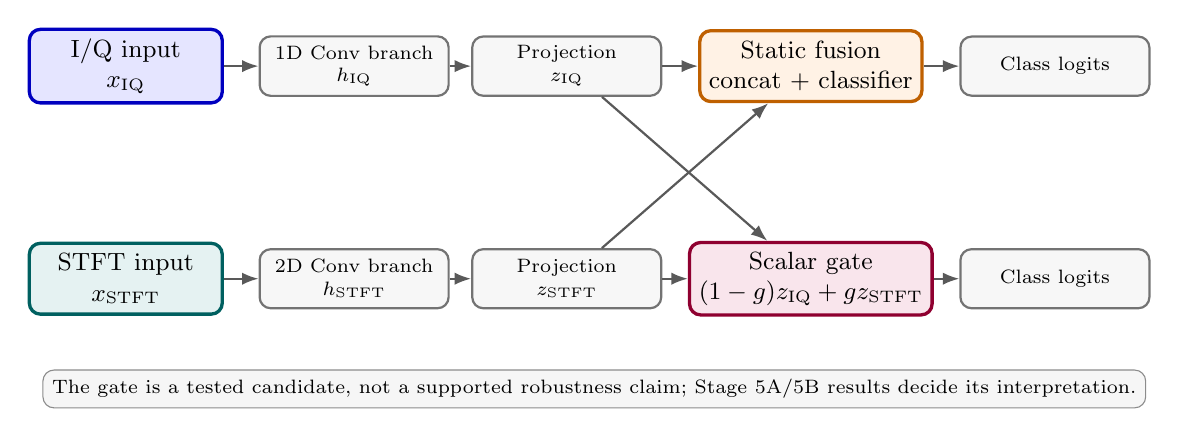
\begin{tikzpicture}[
  block/.style={rounded corners, draw=#1!75!black, fill=#1!10, very thick,
    align=center, minimum width=2.45cm, minimum height=0.9cm, font=\small},
  smallblock/.style={rounded corners, draw=black!55, fill=black!3, thick,
    align=center, minimum width=2.4cm, minimum height=0.75cm, font=\scriptsize},
  arrow/.style={-{Latex[length=2.1mm]}, thick, draw=black!65}
]
\node[block=blue] (iqin) at (0,1.35) {I/Q input\\$x_{\mathrm{IQ}}$};
\node[smallblock] (iqbranch) at (2.9,1.35) {1D Conv branch\\$h_{\mathrm{IQ}}$};
\node[block=teal] (stftin) at (0,-1.35) {STFT input\\$x_{\mathrm{STFT}}$};
\node[smallblock] (stftbranch) at (2.9,-1.35) {2D Conv branch\\$h_{\mathrm{STFT}}$};
\node[smallblock] (proj1) at (5.6,1.35) {Projection\\$z_{\mathrm{IQ}}$};
\node[smallblock] (proj2) at (5.6,-1.35) {Projection\\$z_{\mathrm{STFT}}$};
\node[block=orange] (concat) at (8.7,1.35) {Static fusion\\concat + classifier};
\node[block=purple] (gate) at (8.7,-1.35) {Scalar gate\\$(1-g)z_{\mathrm{IQ}}+gz_{\mathrm{STFT}}$};
\node[smallblock] (out1) at (11.8,1.35) {Class logits};
\node[smallblock] (out2) at (11.8,-1.35) {Class logits};
\draw[arrow] (iqin) -- (iqbranch);
\draw[arrow] (stftin) -- (stftbranch);
\draw[arrow] (iqbranch) -- (proj1);
\draw[arrow] (stftbranch) -- (proj2);
\draw[arrow] (proj1) -- (concat);
\draw[arrow] (proj2) -- (concat);
\draw[arrow] (concat) -- (out1);
\draw[arrow] (proj1) -- (gate);
\draw[arrow] (proj2) -- (gate);
\draw[arrow] (gate) -- (out2);
\node[draw=black!45, rounded corners, fill=gray!7, align=center, font=\scriptsize,
  minimum width=11.7cm] at (5.95,-2.75)
  {The gate is a tested candidate, not a supported robustness claim; Stage 5A/5B results decide its interpretation.};
\end{tikzpicture}%
}

  \caption{静态 I/Q--STFT 融合与标量门控融合结构对比。静态融合直接拼接两分支嵌入（\(\mathbb{R}^{128+64}\)）；门控融合先投影至公共维度（\(\mathbb{R}^{128}\)），再以样本级标量权重组合。}
  \label{fig:fusion-architecture}
\end{figure}

\section{提案模型与训练侧干预}\label{sec:method-proposed}

\subsection{架构动机}

第~\ref{sec:results-extended}~节乘加量分析显示，\texttt{fusion\_iq\_stft} 的 I/Q 分支 MACs 仅 2.0 M，而 \texttt{resnet1d} 为 4.9 M；换言之，``融合输给 CLDNN'' 更可能源于 I/Q 表征容量不足，而非多视图结构本身的局限。基于此，提案模型 \texttt{fusion\_cldnn\_stft} 将 I/Q 分支替换为 \texttt{CLDNNIQBranch}——与 \texttt{cldnn} 共享卷积特征栈（Conv1d 64-128-128ch）加单层 LSTM\cite{sainath2015cldnn,hochreiter1997lstm}，取末时刻隐状态 \(h_T\) 为分支嵌入；STFT 分支沿用 \texttt{TimeFrequencyBranch2D}（与 \texttt{tfcnn\_stft} 结构相同\cite{ioffe2015batchnorm}），分类头为小型 MLP\cite{srivastava2014dropout}：
\begin{equation}
  h_{\mathrm{IQ}}=\mathrm{LSTM}\bigl(f_{\mathrm{1D}}(x_{\mathrm{IQ}})\bigr)_T,\quad
  h_{\mathrm{STFT}}=f_{\mathrm{2D}}(x_{\mathrm{STFT}}),\quad
  \hat{y}=\mathrm{MLP}_2\!\bigl([h_{\mathrm{IQ}}\,\|\,h_{\mathrm{STFT}}]\bigr).
  \label{eq:fusion-cldnn-stft}
\end{equation}
模型总参数量 286 k（介于 \texttt{cldnn} 的 241.7 k 与 \texttt{mcldnn} 的 406.2 k 之间），逐层结构见表~\ref{tab:fusion-cldnn-stft-arch}。

\begin{table}[htbp]
  \centering
  \caption{提案模型 \texttt{fusion\_cldnn\_stft} 逐层结构（batch=1，形状按各分支独立标记）}
  \label{tab:fusion-cldnn-stft-arch}
  \small
  \begin{tabular}{llll}
    \toprule
    分支 / 层 & 操作 & 输出形状 & 说明 \\
    \midrule
    \multicolumn{4}{l}{\textit{I/Q 分支 (\texttt{CLDNNIQBranch})}} \\
    \quad Conv1d-1  & kernel 7, padding 3, 64ch, BN, ReLU  & \([64,128]\) & --- \\
    \quad MaxPool1d & kernel 2                               & \([64, 64]\) & --- \\
    \quad Conv1d-2  & kernel 5, padding 2, 128ch, BN, ReLU & \([128,64]\) & --- \\
    \quad MaxPool1d & kernel 2                               & \([128,32]\) & --- \\
    \quad Conv1d-3  & kernel 3, padding 1, 128ch, BN, ReLU & \([128,32]\) & --- \\
    \quad LSTM      & hidden=128, 1 层, 取 \(h_T\)         & \([128]\)    & batch\_first \\
    \midrule
    \multicolumn{4}{l}{\textit{STFT 分支 (\texttt{TimeFrequencyBranch2D})}} \\
    \quad Conv2d-1  & kernel 3, padding 1, 16ch, BN, ReLU  & \([16,32,7]\) & --- \\
    \quad MaxPool2d & kernel 2                               & \([16,16,3]\) & --- \\
    \quad Conv2d-2  & kernel 3, padding 1, 32ch, BN, ReLU  & \([32,16,3]\) & --- \\
    \quad MaxPool2d & kernel 2                               & \([32, 8,1]\) & --- \\
    \quad Conv2d-3  & kernel 3, padding 1, 64ch, BN, ReLU  & \([64, 8,1]\) & --- \\
    \quad AvgPool   & AdaptiveAvgPool2d(1), flatten          & \([64]\)      & --- \\
    \midrule
    \multicolumn{4}{l}{\textit{融合分类头}} \\
    \quad Concat    & \([128]\,\|\,[64]\)                   & \([192]\)    & --- \\
    \quad Linear-1  & \(192\to192\), ReLU, Dropout(0.1)    & \([192]\)    & --- \\
    \quad Linear-2  & \(192\to11\)                          & \([11]\)     & --- \\
    \bottomrule
  \end{tabular}
\end{table}

\subsection{信号域增强}

信号域增强仅在训练集启用，以保留 I/Q 物理可解释性。本文采用两种变换：

\textbf{随机相位旋转。}以概率 0.5 对每个训练样本施加角度 \(\theta\sim\mathcal{U}[0,2\pi)\) 的相位旋转：
\begin{equation}
  \begin{bmatrix}I'[n]\\Q'[n]\end{bmatrix}
  =\begin{bmatrix}\cos\theta & -\sin\theta\\\sin\theta & \cos\theta\end{bmatrix}
  \begin{bmatrix}I[n]\\Q[n]\end{bmatrix},\quad n=0,\ldots,127.
  \label{eq:phase-rotation}
\end{equation}
相位旋转保持各调制信号的星座图结构，不改变有效 SNR，分类标签不变。

\textbf{随机循环时移。}以概率 0.5 对样本施加随机整数时移 \(k\sim\mathcal{U}\{-32,\ldots,+32\}\)：
\begin{equation}
  I'[n]=I[(n-k)\bmod 128],\quad Q'[n]=Q[(n-k)\bmod 128].
  \label{eq:cyclic-shift}
\end{equation}
循环时移扩充序列对齐多样性，不影响频域特征分布，有效 SNR 与分类标签不变。

幅度缩放与加性高斯噪声因改变有效 SNR 而不予采用；图像式 mixup 因对 I/Q 线性插值缺乏物理可解释性\cite{huang2022mixingsignals,shorten2019dataaug}也不采用。图~\ref{fig:augmentation-demo} 给出四种情形的波形可视化对比。

\subsection{标签平滑}

标签平滑 \(\epsilon=0.1\)\cite{szegedy2016inception} 将 one-hot 目标 \(\mathbf{1}_{y}\) 替换为软目标分布：
\begin{equation}
  q_k=\begin{cases}1-\varepsilon+\varepsilon/K & k=y,\\
  \varepsilon/K & k\neq y,\end{cases}
  \quad K=11.
  \label{eq:label-smoothing}
\end{equation}
该操作抑制过度自信，是分类任务的常见正则化手段，在本实验中由 \texttt{train.loss} 字段配置。

\subsection{三项干预的不平等贡献}\label{sec:method-ablation-preview}

三项干预对整体准确率的贡献并不对等：消融实验（第~\ref{sec:proposed-ablation}~节）显示，架构升级本身对整体准确率的增益约 0 pp（相对 \texttt{cldnn} 仅 \(-0.13\) pp，在种子噪声范围内）；信号域增强是主要贡献项，净增益约 \(+1.55\) pp（arch+aug vs. arch\_only，McNemar \(p\approx6\times10^{-78}\)）；标签平滑则略有负效（\(-0.19\) pp，95\% CI $[-0.0033,-0.0006]$，\(p=0.0155\)）。因此，提案模型的实质贡献应理解为"验证信号域增强在卷积-循环融合架构上的有效性"，架构升级与标签平滑均非主要来源。

\begin{figure}[htbp]
  \centering
  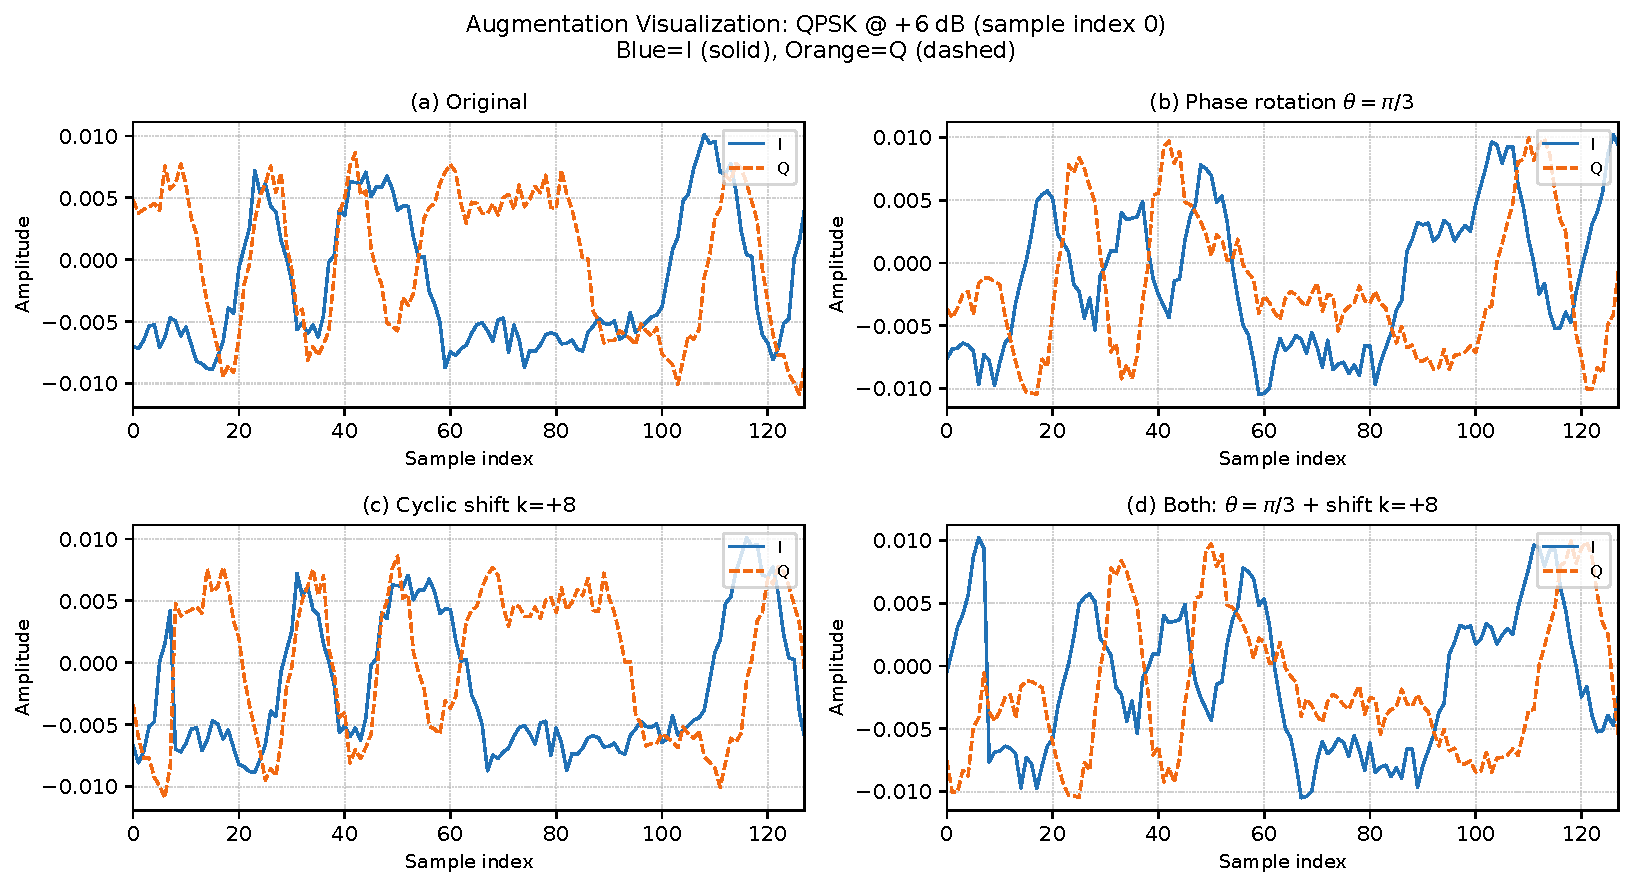
\includegraphics[width=0.96\textwidth]{fig23_augmentation_visualization.pdf}
  \caption{信号域增强示例（QPSK @ +6 dB 单样本）。(a) 原始；(b) 相位旋转 $\theta=\pi/3$；(c) 循环时移 $k=+8$；(d) 两者叠加。I/Q 通道线型见图例。}
  \label{fig:augmentation-demo}
\end{figure}

\section{实现细节与比较纪律}\label{sec:method-impl}

所有模型使用 PyTorch~2.9.1+cu128\cite{paszke2019pytorch} 与 NVIDIA driver 570.\(\ast\) 实现，数据集固定划分（训练/验证/测试集一次性确定，全程不变）。主实验 9 个模型行在 RTX 4070 Ti (Ada, sm\_89) 上训练；提案模型及消融变体在 RTX 3090 (Ampere, sm\_86) 上训练。两批实验的硬件差异作为协议混淆因素显式登记，不参与跨批直接数值比较。

共用训练设置：优化器 AdamW\cite{loshchilov2019adamw,kingma2015adam}，学习率 \(\eta=10^{-3}\)（AMC 卷积网络的常用设定\cite{xu2020mcldnn,zhang2021petcgdnn}），权重衰减 \(10^{-4}\)\cite{krogh1992weightdecay}，批量大小 256。主实验矩阵最大训练轮数 30，早停耐心值 8（依据验证集准确率）；提案模型及消融变体最大轮数 50，早停耐心值 15，额外采用 5 轮线性 warmup 加 cosine annealing 学习率调度\cite{loshchilov2017sgdr}。损失函数默认为标准交叉熵；提案模型加 \(\varepsilon=0.1\) 标签平滑（式~\ref{eq:label-smoothing}）。所有模型以种子集合 \{42, 2025, 3407\} 各训练一次，报告均值 \(\pm\) 标准差。

统一超参作用于主实验矩阵全部 9 个模型，不做模型级事后调参，以保持比较纪律。提案模型及消融变体独立评估，结论限于第~\ref{sec:proposed-ablation}~节范围内，不与主实验矩阵做直接数值比较。本章方法描述限定于已登记模型与训练设置，不引入未在第~4~章评估的诊断性候选。

\chapter{实验结果与统计检验}

\section{写作占位}

本章为实验结果与统计检验占位。正式正文应从主表、low-SNR 表、paired bootstrap 和 McNemar 检验组织结果：CLDNN 的固定协议内 overall 表现、static fusion 的 low-SNR trade-off、gated fusion 的负结果、受控 CUDA latency 对比，以及 MCLDNN retained negative evidence。

\section{声明边界}

本章不得重建主表，不得运行或混入新实验，不得把 confidence interval 或 McNemar 结果外推到未测试数据集。Stage 6B smoke/diagnostic 只能作为排除项出现，不得进入结果表、图或结论。

\chapter{讨论、局限性与可复现性}

\section{固定协议下结果的含义}

第~4~章结果表明，CLDNN 在本文固定协议中取得最高的整体准确率和宏平均 F1，并在已登记配对检验中优于 \path{resnet1d} 与 \path{iq_param_matched}。这一现象可以从结构上理解：CLDNN 先用卷积层提取局部时域模式，再通过循环单元建模序列依赖，相比单纯一维卷积基线具有更强的时序表征能力。与此同时，CLDNN 的优势仍然是协议内观察，不能扩展为跨数据集或跨信道条件的普遍结论。

固定划分的价值在于提高模型间比较的可比性。所有模型使用相同测试样本、相同训练种子集合和相同评价脚本，因而结果差异更容易归因于当前模型实现与训练配置，而不是测试集变化。其限制也同样明显：单一固定划分不能替代多划分重复实验，也不能证明模型对其他数据集或真实无线环境具有相同表现。

\section{STFT 融合的低信噪比权衡}

静态 I/Q--STFT 融合的结果说明，多视图输入的价值具有条件性。相对参数匹配 I/Q 控制模型，静态融合在低信噪比范围内有小幅正向差异；相对 CLDNN，该差异没有统计支持；在整体测试集上，静态融合又低于参数匹配 I/Q 控制模型。因此，本文只能得出“STFT 视图在低信噪比样本上可能提供局部补充信息”的保守结论。

这种权衡具有合理机制解释。低信噪比下，原始 I/Q 序列中的局部相位和幅度结构容易被噪声扰动，STFT 展开的局部频率能量分布可能提供另一种观察角度。但在中高信噪比样本上，I/Q 序列已经包含较清晰的时域判别线索，额外的时频分支和融合分类器可能引入训练难度、特征冗余或视图不一致，从而造成整体准确率下降。由此可见，融合结构的关键问题不是“是否增加视图”，而是如何在低信噪比收益与中高信噪比保持之间取得平衡。

\section{门控融合负结果的意义}

门控融合没有改善静态融合，是本文值得保留的负结果。该模型的设计动机是用样本级标量门控自动调节 I/Q 与 STFT 表征贡献，但当前结果显示，门控权重并未带来更好的整体或低信噪比表现。可能原因包括：门控输入没有显式信噪比信息，标量权重难以表达复杂的类别和信噪比依赖关系；门控子网络也可能在有限训练协议下增加优化难度。

这一负结果不应被解释为所有注意力或门控机制都无效。它只说明本文登记的 \path{gated_fusion_iq_stft}、当前实现和当前训练协议没有形成预期收益。后续若研究显式信噪比感知门控、类别条件门控或更稳定的多视图训练策略，应以新的协议独立评估，不能把设想直接写成本报告结论。

\section{MCLDNN 异常的解释边界}

MCLDNN 的两个训练种子出现近似随机水平的单类预测，说明该结构在当前实现和训练配置下存在明显稳定性问题。保留异常种子并不是降低报告质量，而是维护固定协议的一致性：如果只删除失败种子，主表会变得更好看，但不再忠实反映登记实验矩阵。

该异常更适合解释为优化或初始化敏感性，而不是直接证明数据错误或模型家族无效。已有审计材料没有提供删除种子的证据，因此本文保留完整三种子聚合。后续若要修复或诊断 MCLDNN，应使用新的模型标识、独立输出目录和完整统计检验，不能用诊断性结果替换本文主表。

\section{复杂度与运行时证据限制}

本文的复杂度讨论只覆盖参数量、训练时间背景和受控 CUDA 前向延迟。该测量能帮助读者理解不同模型在相同硬件和相同计时设置下的前向耗时差异，但不能代表完整部署成本。尤其对于 STFT 和 I/Q--STFT 模型，当前延迟表不包含完整时频预处理、数据搬运、CPU 推理或端到端流水线时间。

因此，本文不作“更适合部署”“更高计算效率”或“硬件可迁移性能更好”的判断。若未来需要系统级效率分析，应同时测量 CPU/GPU、不同批量大小、预处理耗时、内存峰值、吞吐率和端到端延迟，并将该协议与本报告的受控前向延迟区分开。

\section{可复现性与证据边界}

本文可复现性主要来自三个层面：固定划分和三训练种子保证比较口径一致；测试集预测归档支持同一样本上的配对统计检验；聚合表、低信噪比分组表和受控延迟表使正文数值可追溯。表~\ref{tab:course-artifact-boundary} 用课程论文口径概括这些材料的用途，具体路径、环境和同步状态放在附录 A。

\begin{table}[htbp]
  \centering
  \caption{课程报告使用的主要证据材料及边界}
  \label{tab:course-artifact-boundary}
  \begin{tabularx}{\textwidth}{lXX}
    \toprule
    材料类型 & 主要作用 & 使用边界 \\
    \midrule
    聚合结果表 & 支撑主结果、低/中/高信噪比分组和复杂度背景。 & 只用于 \datasetname{} 固定协议，不外推到其他数据集。 \\
    测试集预测归档 & 支撑配对自助法和 McNemar 检验。 & 只覆盖 9 个模型行、3 个训练种子和已登记模型对。 \\
    受控延迟表 & 支撑参数量与 CUDA 前向延迟讨论。 & 不代表 CPU、预处理完整耗时或端到端部署成本。 \\
    环境与同步记录 & 说明本地写作环境、服务器实验环境和权重归档缺口。 & 不等同于本地完整训练权重归档。 \\
    \bottomrule
  \end{tabularx}
\end{table}

附录图~\ref{fig:evidence-boundary} 进一步说明证据标签与排除规则。诊断性或工程检查材料可以用于说明后续工作边界，但不能进入主结果、统计检验、摘要和结论。当前本地材料足以支撑报告写作和统计解释，但并不包含完整 27 个训练权重文件；若未来需要模型加载或权重级复现，应先进行独立权重同步和哈希核验。

\chapter{总结}

\section{写作占位}

本章为总结占位。正式正文应以课程报告语气概括：本工作完成了固定协议下的模型矩阵比较、统计检验和证据归档；主要结论必须保持 protocol-bounded。

\section{声明边界}

总结只能回收正文已经由 evidence source 支撑的结论。不得新增 SOTA、跨数据集、广义融合优越性、部署优越性或 Stage 6B 诊断结果主实验化表述。


\begin{reference}
  \printbibliography[heading=none]
\end{reference}

\appendix
\chapter{证据包与实验环境}

\section{写作占位}

本附录为证据包与实验环境占位。正式正文应列出 paper package、predictions archive、statistical-test package、manifest、hash 状态、服务器环境、本地环境，以及 Stage 6B smoke/diagnostic 排除规则。

\section{声明边界}

附录只记录证据来源与复现边界，不写新的实验发现。若后续需要列命令，应明确标注为既有 artifact 追溯或未来复现准备，不能暗示本轮运行过训练、tiny subset、RadioML2018.01A 或 LaTeX 编译。

\chapter{完整训练超参表}
\label{appendix:hyperparameters}

为便于复现，本附录列出本报告所有训练运行的完整超参，按证据标签分组。所有超参在配置文件中均显式给出（路径见每段末），训练代码与种子参考第~3~章实现细节。

\section{Stage 5A 主表（PROJECT\_SUPPORTED, RTX 4070）}

\begin{tabularx}{\textwidth}{lX}
\toprule
项 & 值 \\
\midrule
最大轮数 & 30 \\
批量大小 & 256 \\
优化器 & AdamW (\(\beta_1=0.9, \beta_2=0.999, \varepsilon=10^{-8}\)) \\
学习率 & \(10^{-3}\)（不退火，恒定） \\
权重衰减 & \(10^{-4}\) \\
早停耐心值 & 8（依据验证准确率） \\
学习率调度 & 无（恒定） \\
损失 & 标准交叉熵（\(\epsilon=0\)） \\
增强 & 无 \\
设备 & RTX 4070 (Ada sm\_89), CUDA 12.8, PyTorch 2.9.1+cu128 \\
配置文件 & \path{configs/paper/rml2016a_main_table_full_template.yaml} \\
\bottomrule
\end{tabularx}

\section{扩展训练预算（EXTENDED\_BUDGET\_3090, RTX 3090）}

\begin{tabularx}{\textwidth}{lX}
\toprule
项 & 值 \\
\midrule
最大轮数 & 50 \\
批量大小 & 256 \\
优化器 & AdamW \\
学习率 & 初始 \(10^{-3}\) \\
学习率调度 & 5 轮线性 warmup + cosine annealing 至 0 \\
权重衰减 & \(10^{-4}\) \\
早停耐心值 & 15 \\
损失 & 标准交叉熵 \\
增强 & 无 \\
设备 & RTX 3090 (Ampere sm\_86), CUDA 12.8, PyTorch 2.9.1+cu128 \\
模型范围 & \path{cnn1d}, \path{resnet1d}, \path{iq_param_matched}, \path{fusion_iq_stft} \\
配置文件 & \path{configs/paper/rml2016a_extended_budget_3090.yaml} \\
\bottomrule
\end{tabularx}

\section{低信噪比加权交叉熵（LOW\_SNR\_WEIGHTED\_CE\_3090, RTX 3090）}

\begin{tabularx}{\textwidth}{lX}
\toprule
项 & 值 \\
\midrule
基础设置 & 同上 EXTENDED\_BUDGET\_3090 \\
损失 & 分组 SNR 加权交叉熵；权重 \(w_{\text{low}}=2.0,\ w_{\text{mid}}=1.0,\ w_{\text{high}}=0.7\) \\
SNR 边界 & low\(\le -6\) dB；mid \(\in[-4,6]\) dB；high \(\ge 8\) dB \\
模型范围 & \path{cldnn}, \path{fusion_iq_stft} \\
配置文件 & \path{configs/paper/rml2016a_low_snr_weighted_ce_3090.yaml} \\
\bottomrule
\end{tabularx}

\section{扩展复杂度与 CPU 延迟（CONTROLLED\_LATENCY\_EXTENDED, EPYC CPU）}

\begin{tabularx}{\textwidth}{lX}
\toprule
项 & 值 \\
\midrule
设备 & AMD EPYC 7B12, 强制 \texttt{torch.set\_num\_threads(1)} \\
预热迭代 & 50 \\
计时迭代 & 200 \\
批量大小 & 1 与 256（两次单独测量） \\
PyTorch & 2.9.1+cu128（仅作前向传播，CPU 后端） \\
脚本 & \path{scripts/paper/measure_extended_complexity_latency.py} \\
\bottomrule
\end{tabularx}

\section{提案模型 + 增强 + 标签平滑（FUSION\_CLDNN\_STFT\_AUG\_LS\_3090, RTX 3090）}

\begin{tabularx}{\textwidth}{lX}
\toprule
项 & 值 \\
\midrule
基础设置 & 同上 EXTENDED\_BUDGET\_3090 \\
损失 & 标签平滑交叉熵, \(\epsilon=0.1\) \\
增强（仅训练集） & 相位旋转 \(\theta\sim\mathcal{U}(-\pi,\pi)\), prob 0.5；循环时移 \(k\sim\mathcal{U}(-8,+8)\), prob 0.5 \\
模型 & \path{fusion_cldnn_stft}（CLDNN 风格 I/Q 编码器 + STFT 二维分支 + 融合 MLP 头） \\
模型参数量 & 286,331 \\
配置文件 & \path{configs/paper/rml2016a_fusion_cldnn_stft_aug_ls_3090.yaml} \\
\bottomrule
\end{tabularx}

\section{提案模型单干预消融（FUSION\_CLDNN\_STFT\_ABLATION\_3090, RTX 3090）}

\begin{tabularx}{\textwidth}{lX}
\toprule
项 & 值 \\
\midrule
基础设置 & 同上 FUSION\_CLDNN\_STFT\_AUG\_LS\_3090（3 变体共享） \\
变体 \texttt{arch\_only} & 增强 OFF, \(\epsilon=0\)（纯架构升级） \\
变体 \texttt{arch\_aug}  & 增强 ON,  \(\epsilon=0\) \\
变体 \texttt{arch\_ls}   & 增强 OFF, \(\epsilon=0.1\) \\
模型 & \path{fusion_cldnn_stft}（与上一节相同实现） \\
配置文件 & \path{configs/paper/rml2016a_fusion_cldnn_stft_ablation_3090.yaml} \\
\bottomrule
\end{tabularx}

\section{固定划分与训练种子（所有标签共用）}

\begin{tabularx}{\textwidth}{lX}
\toprule
项 & 值 \\
\midrule
固定划分 & \splitname{} 加密保存为 NPZ 数组 \\
划分文件 & \path{data/splits/rml2016a/stratified_by_mod_snr_seed42.npz} \\
划分摘要 & \path{data/splits/rml2016a/stratified_by_mod_snr_seed42_summary.json} \\
分层维度 & 调制方式 \(\times\) 信噪比联合分层（11 \(\times\) 20 = 220 个组） \\
切分比例 & 70\% / 10\% / 20\% (训练 / 验证 / 测试) \\
切分种子 & 42 \\
训练种子 & 42, 2025, 3407（3 个） \\
\bottomrule
\end{tabularx}

\end{document}
